\documentclass[12pt]{article}
\usepackage[utf8]{inputenc}
\usepackage[spanish]{babel}
\usepackage{amsmath}
\usepackage{amsthm}
\usepackage{multicol,multienum}
\usepackage{graphicx}
\usepackage{standalone}
\usepackage[outdir=../]{epstopdf}
\usepackage[binary-units=true]{siunitx}
\usepackage{float}
\DeclareGraphicsExtensions{.pdf,.png,.jpg}
\usepackage{tikz}
\usetikzlibrary{patterns}
\usetikzlibrary{decorations.pathmorphing,patterns}
\usetikzlibrary{arrows,calc,patterns,decorations.markings}
\usetikzlibrary{positioning}
\usepackage{color}
\usepackage{anysize}
\usepackage[spanish=mexican]{csquotes}
\usepackage{anyfontsize}
\usepackage[os=win]{menukeys}
\usepackage{pbox}
%Este paquete permite manejar los encabezados del documento
\usepackage{fancyhdr}
%hay que definir el ambiente de la página
\pagestyle{fancy}
%aqui va el texto para todas las paginas l--> izquierda, r--> derecha, hay un C--> para centrar el texto deseado
%\lhead{Curso de Física Computacional}
\fancyhead[R]{\nouppercase{\leftmark}}
%define el ancho de la linea que separa el encabezado del cuerpo del texto
\renewcommand{\headrulewidth}{0.5pt}
\setlength{\parskip}{1em}
\renewcommand{\baselinestretch}{1.25}
\newcommand{\python}{\texttt{python}}
\newcommand{\funcionazul}[1]{\textcolor{blue}{\textbf{\texttt{#1}}}}
\interfootnotelinepenalty=8000
\usepackage{hyperref}
%esta parte define el color del marco que aparece en las hiperreferencias.
\definecolor{links}{HTML}{2A1B81}
\hypersetup{colorlinks,linkcolor=,urlcolor=links}
\spanishdecimal{.}
\marginsize{1.5cm}{1.5cm}{1.5cm}{1.5cm}
\numberwithin{equation}{section}
\date{}
\usepackage{listings}
\usepackage{xcolor}
\usepackage{textcomp}
\usepackage{color}
\definecolor{deepblue}{rgb}{0,0,0.5}
\definecolor{brown}{rgb}{0.59, 0.29, 0.0}
\definecolor{OliveGreen}{rgb}{0,0.25,0}
% \usepackage{minted}

% \DeclareCaptionFont{white}{\color{white}}
% \DeclareCaptionFormat{listing}{\colorbox{gray}{\parbox{0.98\textwidth}{#1#2#3}}}
% \captionsetup[lstlisting]{format=listing,labelfont=white,textfont=white}
\renewcommand{\lstlistingname}{Código}


\definecolor{Code}{rgb}{0,0,0}
\definecolor{Keywords}{rgb}{255,0,0}
\definecolor{Strings}{rgb}{255,0,255}
\definecolor{Comments}{rgb}{0,0,255}
\definecolor{Numbers}{rgb}{255,128,0}



\lstset{ 
language=Python,                % choose the language of the code
basicstyle=\normalsize\ttfamily,       % the size of the fonts that are used for the code
numbers=left,                   % where to put the line-numbers
numberstyle=\scriptsize,      % the size of the fonts that are used for the line-numbers
stepnumber=1,                   % the step between two line-numbers. If it is 1 each line will be numbered
numbersep=5pt,                  % how far the line-numbers are from the code
backgroundcolor=\color{white},  % choose the background color. You must add \usepackage{color}
showspaces=false,               % show spaces adding particular underscores
showstringspaces=false,         % underline spaces within strings
showtabs=false,                 % show tabs within strings adding particular underscores
frame=single,   		% adds a frame around the code
tabsize=2,  		% sets default tabsize to 2 spaces
captionpos=t,   		% sets the caption-position to bottom
breaklines=true,    	% sets automatic line breaking
breakatwhitespace=false,    % sets if automatic breaks should only happen at whitespace
escapeinside={\#},  % if you want to add a comment within your code
stringstyle =\color{OliveGreen},
%otherkeywords={{as}},             % Add keywords here
keywordstyle = \color{blue},
commentstyle = \color{black},
identifierstyle = \color{black},
literate=%
         {á}{{\'a}}1
         {é}{{\'e}}1
         {í}{{\'i}}1
         {ó}{{\'o}}1
         {ú}{{\'u}}1
%
%keywordstyle=\ttb\color{deepblue}
%fancyvrb = true,
}

\lstdefinestyle{FormattedNumber}{%
    literate={0}{{\textcolor{red}{0}}}{1}%
             {1}{{\textcolor{red}{1}}}{1}%
             {2}{{\textcolor{red}{2}}}{1}%
             {3}{{\textcolor{red}{3}}}{1}%
             {4}{{\textcolor{red}{4}}}{1}%
             {5}{{\textcolor{red}{5}}}{1}%
             {6}{{\textcolor{red}{6}}}{1}%
             {7}{{\textcolor{red}{7}}}{1}%
             {8}{{\textcolor{red}{8}}}{1}%
             {9}{{\textcolor{red}{9}}}{1}%
             {.0}{{\textcolor{red}{.0}}}{2}% Following is to ensure that only periods
             {.1}{{\textcolor{red}{.1}}}{2}% followed by a digit are changed.
             {.2}{{\textcolor{red}{.2}}}{2}%
             {.3}{{\textcolor{red}{.3}}}{2}%
             {.4}{{\textcolor{red}{.4}}}{2}%
             {.5}{{\textcolor{red}{.5}}}{2}%
             {.6}{{\textcolor{red}{.6}}}{2}%
             {.7}{{\textcolor{red}{.7}}}{2}%
             {.8}{{\textcolor{red}{.8}}}{2}%
             {.9}{{\textcolor{red}{.9}}}{2}%
             {\ }{{ }}{1}% handle the space
         ,%
          %mathescape=true
          escapeinside={__}
}

\title{Métodos directos de solución para problemas matriciales \\ \begin{Large}Curso de Física Computacional - Guía de apoyo \end{Large}}
\author{M. en C. Gustavo Contreras Mayén.}
%\usepackage{listings}
\usepackage{xcolor}
\usepackage{textcomp}
\usepackage{color}
\definecolor{deepblue}{rgb}{0,0,0.5}
\definecolor{brown}{rgb}{0.59, 0.29, 0.0}
\definecolor{OliveGreen}{rgb}{0,0.25,0}
% \usepackage{minted}

% \DeclareCaptionFont{white}{\color{white}}
% \DeclareCaptionFormat{listing}{\colorbox{gray}{\parbox{0.98\textwidth}{#1#2#3}}}
% \captionsetup[lstlisting]{format=listing,labelfont=white,textfont=white}
\renewcommand{\lstlistingname}{Código}


\definecolor{Code}{rgb}{0,0,0}
\definecolor{Keywords}{rgb}{255,0,0}
\definecolor{Strings}{rgb}{255,0,255}
\definecolor{Comments}{rgb}{0,0,255}
\definecolor{Numbers}{rgb}{255,128,0}



\lstset{ 
language=Python,                % choose the language of the code
basicstyle=\normalsize\ttfamily,       % the size of the fonts that are used for the code
numbers=left,                   % where to put the line-numbers
numberstyle=\scriptsize,      % the size of the fonts that are used for the line-numbers
stepnumber=1,                   % the step between two line-numbers. If it is 1 each line will be numbered
numbersep=5pt,                  % how far the line-numbers are from the code
backgroundcolor=\color{white},  % choose the background color. You must add \usepackage{color}
showspaces=false,               % show spaces adding particular underscores
showstringspaces=false,         % underline spaces within strings
showtabs=false,                 % show tabs within strings adding particular underscores
frame=single,   		% adds a frame around the code
tabsize=2,  		% sets default tabsize to 2 spaces
captionpos=t,   		% sets the caption-position to bottom
breaklines=true,    	% sets automatic line breaking
breakatwhitespace=false,    % sets if automatic breaks should only happen at whitespace
escapeinside={\#},  % if you want to add a comment within your code
stringstyle =\color{OliveGreen},
%otherkeywords={{as}},             % Add keywords here
keywordstyle = \color{blue},
commentstyle = \color{black},
identifierstyle = \color{black},
literate=%
         {á}{{\'a}}1
         {é}{{\'e}}1
         {í}{{\'i}}1
         {ó}{{\'o}}1
         {ú}{{\'u}}1
%
%keywordstyle=\ttb\color{deepblue}
%fancyvrb = true,
}

\lstdefinestyle{FormattedNumber}{%
    literate={0}{{\textcolor{red}{0}}}{1}%
             {1}{{\textcolor{red}{1}}}{1}%
             {2}{{\textcolor{red}{2}}}{1}%
             {3}{{\textcolor{red}{3}}}{1}%
             {4}{{\textcolor{red}{4}}}{1}%
             {5}{{\textcolor{red}{5}}}{1}%
             {6}{{\textcolor{red}{6}}}{1}%
             {7}{{\textcolor{red}{7}}}{1}%
             {8}{{\textcolor{red}{8}}}{1}%
             {9}{{\textcolor{red}{9}}}{1}%
             {.0}{{\textcolor{red}{.0}}}{2}% Following is to ensure that only periods
             {.1}{{\textcolor{red}{.1}}}{2}% followed by a digit are changed.
             {.2}{{\textcolor{red}{.2}}}{2}%
             {.3}{{\textcolor{red}{.3}}}{2}%
             {.4}{{\textcolor{red}{.4}}}{2}%
             {.5}{{\textcolor{red}{.5}}}{2}%
             {.6}{{\textcolor{red}{.6}}}{2}%
             {.7}{{\textcolor{red}{.7}}}{2}%
             {.8}{{\textcolor{red}{.8}}}{2}%
             {.9}{{\textcolor{red}{.9}}}{2}%
             {\ }{{ }}{1}% handle the space
         ,%
          %mathescape=true
          escapeinside={__}
}

\begin{document}
\fontsize{14}{14}\selectfont
\maketitle
\section{Método de eliminación de Gauss.}
La eliminación de Gauss es el método más conocido para la solución de ecuaciones simultáneas. Se compone de dos partes:
\begin{enumerate}
\item La fase de eliminación.
\item La fase de solución.
\end{enumerate}
\subsection{Fase de eliminación}
La función de la fase de eliminación es transformar las ecuaciones en la formar $U \: x = c$. Entonces las ecuaciones son resueltas realizando el procedimiento de sustitución hacia atrás.
\par
Con el fin de ilustrar el procedimiento, vamos a resolver el siguiente sistema de ecuaciones
\begin{eqnarray}
4 \: x_{1} - 2 \: x_{2} + x_{3} =& 11 \label{eq:sistgauss1}\\
-2 \: x_{1} + 4 \: x_{2} - 2 \: x_{3} =& -16 \label{eq:sistgauss2} \\
x_{1} - 2 \: x_{2} + 4 \: x_{3} =& 17 \label{eq:sistgauss3}
\end{eqnarray}
La fase de eliminación utiliza solamente una de las operaciones elementales: multiplicar una ecuación (por ejemplo, ecuación $j$) por una constante $\lambda$ y restarla de otra ecuación (ecuación $i$). 
\par
La representación simbólica de esta operación es
\[Eq.(i) \leftarrow Eq.(i) - \lambda \times Eq.(j)\]
La ecuación que se resta, a saber, la $Eq.(j)$, se llama ecuación pivote.
\par
Comenzamos la eliminación eligiendo la Eq.\eqref{eq:sistgauss1} como ecuación pivote y eligiendo los multiplicadores $\lambda$ a fin de eliminar $x_{1}$ a partir de las Ecs. \eqref{eq:sistgauss2} y \eqref{eq:sistgauss3}:
\[ \begin{split}
Eq.\eqref{eq:sistgauss2} \leftarrow& Eq.\eqref{eq:sistgauss2} - (-0.5) \times Eq.\eqref{eq:sistgauss1} \\
Eq.\eqref{eq:sistgauss3} \leftarrow&Eq.\eqref{eq:sistgauss3} - 0.25 \times Eq.\eqref{eq:sistgauss1}
\end{split}\]
Después de esta transformación, las ecuaciones quedan:
\begin{align}
4 \: x_{1} - 2 \: x_{2} + x_{3} =& 11 \label{eq:sistgauss4}\\
3 \: x_{2} -1.5 \: x_{3} =& -10.5 \label{eq:sistgauss5} \\
-1.5 \: x_{2} + 3.75 \: x_{3} =& 14.25 \label{eq:sistgauss6}
\end{align}
Con este procedimiento se completa el primer paso.
\par
Ahora elegimos $Eq. \eqref{eq:sistgauss5}$ como ecuación pivote y eliminamos $x_{2}$ de la $Eq. \eqref{eq:sistgauss6}$:
\[ Eq.\eqref{eq:sistgauss6} \leftarrow Eq.\eqref{eq:sistgauss6} - (-0.5) \times Eq. \eqref{eq:sistgauss5}\]
que nos devuelve
\begin{align}
4 \: x_{1} - 2 \: x_{2} + x_{3} =& 11 \label{eq:sistgauss7} \\
3 \: x_{2} - 1.5 \: x_{3} =& -10.5 \label{eq:sistgauss8} \\
3 \: x_{3} = 9 \label{eq:sistgauss9}
\end{align}
La fase de eliminación está completa. Las ecuaciones iniciales fueron re-emplazadas por un conjunto de ecuaciones equivalentes que pueden resolverse fácilmente por sustitución hacia atrás.
\subsection*{Uso de la matriz aumentada}
La matriz de coeficientes aumentada es un instrumento más conveniente para realizar los cálculos. 
\par
Así, las ecuaciones originales se escribirían
\[ \left[\begin{tabular}{c c c | c }
$4$ & $-2$ & $1$ & $11$	 \\
$-2$ & $4$ & $-2$ & $-16$ \\
$1$ & $-2$ & $4$ & $17$
\end{tabular} \right] \]
Las ecuaciones equivalentes producidas por el primer y segundo paso de la eliminación de Gauss, quedarían como:
\[ \left[\begin{tabular}{c c c | c }
$4$ & $-2$ & $1$ & $11.00$ \\
$0$ & $3$ & $-1.5$ & $-10.50$ \\
$0$ & $-1.5$ & $3.75$ & $14.25$
\end{tabular} \right] \]
\[ \left[\begin{tabular}{c c c | c }
$4$ & $-2$ & $1$ & $11.00$ \\
$0$ & $3$ & $-1.5$ & $-10.50$ \\
$0$ & $0$ & $3$ & $9.00$
\end{tabular} \right] \]
\subsection{Fase de sustitución hacia atrás}
Las incógnitas ahora puede ser calculadas por sustitución hacia atrás. Resolviendo las ecuaciones $\eqref{eq:sistgauss9}$, $\eqref{eq:sistgauss8}$ y $\eqref{eq:sistgauss7}$ en ese orden, se obtiene
\[ \begin{split}
x_{3} =& 9/3 = 3 \\
x_{2} =& (-10.5 + 1.5 \: x-{3})/3 = -2 \\
x_{1} =& (11 + 2 \: x_{2} - x_{3})/4 = 1
\end{split} \]
\subsection{Algoritmo para la eliminación de Gauss}
\subsection*{Fase de eliminación}
Para codificar el algoritmo de la fase de eliminación del método de eliminación.
\par
Supongamos que las primeras $k$ filas de $A$ ya se han transformado a una forma triangular superior. Por lo que la ecuación pivote actual es la $k$-ésima ecuación, y todas las ecuaciones de abajo están para ser transformadas.
\par
Tenamos entonces que la matriz aumentada es:
\[ \begin{bmatrix}
A_{11} & A_{12} & A_{13} & \ldots & A_{1k} & \ldots & A_{ij} & \ldots & A_{1n} & b_{1} \\
0      & A_{22} & A_{23} & \ldots & A_{2k} & \ldots & A_{2j} & \ldots & A_{2n} & b_{2} \\
0      & 0      & A_{33} & \ldots & A_{3k} & \ldots & A_{3j} & \ldots & A_{3n} & b_{3} \\
\vdots & \vdots & \vdots & \vdots & \vdots & \vdots & \vdots & \vdots & \vdots & \vdots \\
0      & 0      & 0      & A_{kk} & \ldots & \ldots & A_{kj} & \ldots & A_{kn} & b_{k} \\
\vdots & \vdots & \vdots & \vdots & \vdots & \vdots & \vdots & \vdots & \vdots & \vdots \\
0      & 0      & 0      & A_{ik} & \ldots & \ldots & A_{ij} & \ldots & A_{in} & b_{i} \\
\vdots & \vdots & \vdots & \vdots & \vdots & \vdots & \vdots & \vdots & \vdots & \vdots \\
0      & 0      & 0      & A_{nk} & \ldots & \ldots & A_{nj} & \ldots & A_{nn} & b_{n} \\
\end{bmatrix}
\]
\subsection*{Operaciones elementales}
Sea la $i$-ésima fila una fila por debajo de la ecuación pivote que será transformada, lo que significa que el elemento $A_{ik}$ se va a eliminar. 
\par
Logramos esto mediante la multiplicación de la fila pivote por $\lambda = A_{ik} / A_{kk}$ y restarlo de la fila $i$-ésima. Los correspondientes cambios en la fila $i$ son
\[ \begin{split}
A_{ij} \leftarrow& A_{ij} - \lambda A_{kj},  \hspace{1cm} j = k, k+1, \ldots,n \\
b_{i} \leftarrow& b_{i} - \lambda b_{k}
\end{split} \]
Para transformar la matriz de coeficientes a una forma triangular superior, los índices $k$ e $i$ en las ecuaciones anteriores debe tener los intervalos $k = 1, 2, \ldots,n-1$ (de la fila pivote), $i = k + 1, k + 2, \ldots,n$ (de la fila que se va a transformar)
El algoritmo para la fase de eliminación ahora se escribe:
\begin{lstlisting}[caption=Eliminación de Gauss, style=FormattedNumber, basicstyle=\linespread{1.1}\ttfamily=\small, columns=fullflexible]
for k in range(0, n-1):
    for i in range(k+1, n):
        if a[i, k] = 0.0:
            lam = a[i, k]/a[k, k]
            a[i, k+_1_:n] = a[i, k+_1_:n] - lam * a[k, k+_1_:n]
            b[i] = b[i] - lam * b[k]
\end{lstlisting}
\subsection*{Consideraciones}
Con el fin de evitar operaciones innecesarias, el algoritmo anterior considera lo siguiente:
\begin{enumerate}
\item Si $A_{ik}$ vale cero, la transformación de la fila $i$ se omite.
\item El índice $j$ en la ecuación de transformación comienza con $k + 1$ en lugar de $k$.
\par
Por lo tanto, $A_{ik}$ no se re-emplaza con cero, pero conserva su valor original.
\par
Como la fase de solución nunca accede a la parte triangular inferior de la matriz de coeficientes, su contenido es irrelevante.
\end{enumerate}
\subsection{Fase de sustitución}
Luego de la eliminación de Gauss, la matriz de aumentada tiene la siguiente forma
\[ \left[ \begin{array}{c | c}
A & b 
\end{array} \right] =
\left[ \begin{array}{c c c c c | c}
A_{11} & A_{12} & A_{13} & \ldots & A_{1n} & b_{1} \\
0      & A_{22} & A_{23} & \ldots & A_{2n} & b_{2} \\
0 	   & 0      & A_{33} & \ldots & A_{3n} & b_{3} \\
\vdots & \vdots & \vdots & \vdots & \vdots & \vdots \\
0      & 0      & 0      & 0      & A_{nn} & b_{n}
\end{array} \right] \]
La última ecuación $A_{nn} x_{n} = b_{n}$ se resuelve primero para obtener
\[ x_{n} = \dfrac{b_{n}}{A_{nn}}\]
Consideremos ahora la etapa de sustitución hacia atrás donde $x_{n}, x_{n-1}, \ldots,x_{k + 1}$ ya han sido calculados (en ese orden), para determinar $x_{k}$ de la $k$-ésima ecuación:
\[ A_{kk} x_{k} + A_{k,k+1} x_{k+1} + \ldots + A_{kn}x_{n} = b_{k}\]
La solución es:
\[ x_{k} = \left( b_{k} - \sum_{j=k+1}^{n} A_{kj}x_{j} \right) \dfrac{1}{A_{kk}}, \hspace{0.4cm} k=n-1,n-2,\ldots,1 \]
Con \python{} tendremos que:
\begin{lstlisting}[caption=Fase de sustitución, style=FormattedNumber, basicstyle=\linespread{1.1}\ttfamily=\small, columns=fullflexible]
for k in range(n-1,-1,-1):
    b[k] = (b[k] - dot(a[k, k+_1_:n], b[k+_1_:n]))/a[k,k]
return b
\end{lstlisting}
\subsection*{Ejercicio}
Resuelve el problema $A \: x=b$, donde
\[ A = \begin{bmatrix}
2 & -3 & -1 \\
3 & 2 & -5 \\
2 & 4 & -1
\end{bmatrix}
\hspace{1cm} b=
\begin{bmatrix}
3 \\
-9 \\
-5
\end{bmatrix} \]
\subsection{La función \funcionazul{gaussElimin}.}
El siguiente código en \python{} implementa las dos fases del procedimiento de eliminación de Gauss:
\begin{lstlisting}[caption=Función gaussElimin, style=FormattedNumber, basicstyle=\linespread{1.1}\ttfamily=\small, columns=fullflexible]
def gaussElimin(a, b):
    n = len(b)

    for k in range(0, n-1):
        for i in range(k+1, n):
            if a[i, k] = 0.0:
                lam = a[i, k]/a[k, k]
                a[i, k+_1_:n] = a[i, k+_1_:n] - lam * a[k, k+_1_:n]
                b[i] = b[i] - lam * b[k]

    for k in range(n-1, -1, -1):
        b[k] = (b[k] - dot(a[k, k+_1_:n], b[k+_1_:n]))/a[k,k]
    
    return b
\end{lstlisting}
Incorporando los arreglos para resolver el problema:
\begin{lstlisting}[caption=Agregando los arreglos, style=FormattedNumber, basicstyle=\linespread{1.1}\ttfamily=\small, columns=fullflexible]
a = array([[2., -3, -1],[3, 2, -5],[2, 4, -1]])
b = array([3., -9, -5])
x = gaussElimin(a, b)

print (x)
\end{lstlisting}
\subsection*{Corroborando el resultado con \texttt{solve}}
Podemos usar \texttt{linalg.solve} para verificar nuestro resultado, hacemos entonces:
\begin{lstlisting}[caption=Usando \funcionazul{linalg.solve}, style=FormattedNumber, basicstyle=\linespread{1.1}\ttfamily=\small, columns=fullflexible]
print (linalg.solve(a,b))
\end{lstlisting}
Pero nos damos cuenta de que el resultado es completamente diferente:
\begin{verbatim}
Solución con la función gaussElimin
[ 0.65306122 -1.14285714  1.73469388]

Usando la función solve
[ 0.39032237 -0.10984011  0.45710386]
\end{verbatim}
Entonces: ¿qué es lo que pasa?
\par
Lo que ocurre es que al llamar la función \funcionazul{gaussElimin(a,b)}, se modifican los valores de las entradas al llevarse a cabo las operaciones elementales, por lo que los arreglos que se usan para la función \funcionazul{linalg.solve(a,b)}, ya son otros arreglos.
\par
Para corregir esta situación, debemos de garantizar que los arreglos a usar en \funcionazul{linalg.solve}, son idénticos a los arreglos iniciales, para ello, hacemos una copia:
\begin{lstlisting}[caption=Ajuste a la solución, style=FormattedNumber, basicstyle=\linespread{1.1}\ttfamily=\small, columns=fullflexible]	
a = array([[2., -3, -1], [3, 2, -5], [2, 4, -1]])
b = array([3., -9, -5])

c = a.copy()
d = b.copy()

print('Solucion con la funcion gaussElimin')
print (gaussElimin(a,b))
print()

print('Solucion con solve')
print (linalg.solve(c,d))
\end{lstlisting}
Y vemos que ambos resultados son los mismos.
\begin{verbatim}
Solución con la función gaussElimin
[ 0.65306122 -1.14285714  1.73469388]

Usando la función solve
[ 0.65306122 -1.14285714  1.73469388]
\end{verbatim}
\subsection{Sistemas de ecuaciones múltiples}
Como ya se ha mencionado, a menudo es necesario resolver sistemas de ecuaciones $\mathbf{A \: x = b}$ para varios vectores constantes.
\par
Sea $m$ dichos vectores constantes, denotados por $\mathbf{b_{1}, b_{2}, \ldots, b_{m}}$ y dejar que los correspondientes vectores solución sean $\mathbf{x_{1}, x_{2}, \ldots, x_{m}}$. 
Escribimos el conjunto de ecuaciones múltiples $\mathbf{A \: X = B}$, donde
\[ \mathbf{X} = \left[ \mathbf{x_{1}} \hspace{0.2cm} \mathbf{x_{2}} \hspace{0.2cm} \ldots \hspace{0.2cm} \mathbf{x_{m}} \right] \]
y
\[ \mathbf{B} = \left[ \mathbf{b_{1}} \hspace{0.2cm} \mathbf{b_{2}} \hspace{0.2cm} \ldots \hspace{0.2cm} \mathbf{b_{m}} \right] \]
son matrices de $n \times m$ cuyas columnas consisten en vectores solución y vectores constantes, respectivamente.
\par
Una manera económica de manejar ecuaciones de este tipo durante la fase de eliminación es incluir todos los $m$ vectores constantes en la matriz de coeficientes aumentada, de modo que se transforman simultáneamente con la matriz de coeficientes.
\par 
Las soluciones son luego obtenidas por sustitución hacia atrás de la manera habitual, un vector a la vez. Tendremos que ajustar el método de Gauss para realizar esta tarea.
\subsection*{Ejercicio}
Resuelve el sistema de ecuaciones $\mathbf{A \: X = B}$, donde:
\[ A = \begin{bmatrix}
2 & 0 & -1 & 0 \\
0 & 1 & 2 & 0 \\
-1 & 2 & 0 & -2 \\
0 & 0 & 1 & -2
\end{bmatrix}
\hspace{1cm} B =
\begin{bmatrix}
1 & 0 \\
0 & 0 \\
0 & 1 \\
0 & 0
\end{bmatrix} \]
\section{Método de Gauss-Jordan}
El método de Gauss-Jordan es esencialmente la eliminación de Gauss llevada a su límite. En el método de eliminación de Gauss, solo las ecuaciones que se encuentran debajo de la ecuación pivote se transforman.
\par
En el método de Gauss-Jordan, la eliminación también se lleva a cabo en ecuaciones por encima de la ecuación de pivote, lo que da como resultado una matriz de coeficientes diagonales.
\par
La principal desventaja de la eliminación de Gauss-Jordan es que implica aproximadamente $n^{3}/2$ operaciones largas, que es $1.5$ veces más, el número requerido con el procedimiento de eliminación de Gauss.
\section{Ejercicios opcionales}
Los siguientes ejercicios se resuelven utilizando lo revisado en esta guía y en las clases, estos ejercicios son opcionales, se tomará en cuenta para el examen parcial 2, entregando todos los ejercicios y en el caso de que estén bien resueltos, aportarán $\mathbf{0.5}$ \textbf{puntos} adicionales a la calificación del examen parcial 2.
\begin{enumerate}
\item Evaluando el determinante, identifica cuáles de las siguientes matrices, son singulares, mal condicionadas o bien condicionadas:
\begin{multicols}{2}
	\begin{enumerate}
		\item $ \mathbf{A} =
				\begin{pmatrix}
					1 & 2 & 3 \\
					2 & 3 & 4 \\
					3 & 4 & 5
				\end{pmatrix} $
		\item $ \mathbf{A} =
				\begin{pmatrix}
					2.11 & -0.80 & 1.72 \\
					-1.84 & 3.03 & 1.29 \\
					-1.57 & 5.25 & 4.30
				\end{pmatrix} $
		\item $ \mathbf{A} =
				\begin{pmatrix}
					2 & -1 & 0 \\
					-1 & 2 & -1 \\
					0 & -1 & 2
				\end{pmatrix} $
		\item $ \mathbf{A} =
				\begin{pmatrix}
					4 & 3 & -1 \\
					7 & -2 & 3 \\
					5 & -18 & 13
				\end{pmatrix} $ 
	\end{enumerate}
\end{multicols}
\item Dada la descomposición $\mathbf{A} = \mathbf{LU}$, calcular $\mathbf{A}$ y $\vert \mathbf{A} \vert$
	 \begin{enumerate}
	 	\item $ \mathbf{L} =
	 			\begin{pmatrix}
	 				1 & 0 & 0 \\
	 				1 & 1 & 0 \\
	 				1 & 5/3 & 1
				\end{pmatrix} \hspace{0.5cm}
				\mathbf{U} =
				\begin{pmatrix}
					1 & 2 & 4 \\
					0 & 3 & 21 \\
					0 & 0 & 0
				\end{pmatrix} $
		\item $ \mathbf{L} =
	 			\begin{pmatrix}
	 				2 & 0 & 0 \\
	 				-1 & 1 & 0 \\
	 				1 & -3 & 1
				\end{pmatrix} \hspace{0.5cm}
				\mathbf{U} =
				\begin{pmatrix}
					2 & -1 & 1 \\
					0 & 1 & -3 \\
					0 & 0 & 1
				\end{pmatrix} $
	 \end{enumerate}
\item Usando los resultados de la descomposición LU
\[  \mathbf{A} =
	\mathbf{LU} =
	\begin{pmatrix}
		1 & 0 & 0 \\
		3/2 & 1  & 0 \\
		1/2 & 11/13 & 1
	\end{pmatrix}
	\begin{pmatrix}
		2 & -3 & -1 \\
		0 & 13/2 & -7/2 \\
		0 & 0 & 32/13
	\end{pmatrix}	 \]
	para resolver $\mathbf{Ax} = \mathbf{b}$, donde $\mathbf{b}^{T} = [1 \hspace{0.3cm} -1 \hspace{0.3cm} 2 ]$.
\item Resolver la ecuación $\mathbf{Ax} = \mathbf{b}$ con el método de eliminación de Gauss, donde
\[  \mathbf{A} =
	\begin{pmatrix}
		0 & 0 & 2 & 1 & 2 \\
		0 & 1 & 0 & 2 & -1 \\
		1 & 2 & 0 & -2 & 0 \\
		0 & 0 & 0 & -1 & 1 \\
		0 & 1 & -1 & 1 & -1
	\end{pmatrix} \hspace{1.5cm}
	\mathbf{b} =	
	\begin{pmatrix}
		1 \\
		1 \\
		-4 \\
		-2 \\
		-1
	\end{pmatrix} \]
\item Encontrar $\mathbf{L}$ y $\mathbf{U}$ tales que:
\[ \mathbf{A} = \mathbf{LU} =
	\begin{pmatrix}
		4 & -1 & 0 \\
		-1 & 4 & -4 \\
		0 & -1 & 4
	\end{pmatrix} \]
	usando a) la descomposición de Doolittle y b) la descomposición de Choleski.
\item Utiliza la descomposición de Doolittle para resolver $\mathbf{Ax}=\mathbf{b}$, donde
\[  \mathbf{A} =
	\begin{pmatrix}
		-3 & 6 & -4 \\
		9 & -8 & 24 \\
		-12 & 24 & -26 \\
	\end{pmatrix} \hspace{1.5cm}
	\mathbf{b} =	
	\begin{pmatrix}
		-3 \\
		65 \\
		-42
	\end{pmatrix} \]
\item Resolver $\mathbf{Ax} = \mathbf{b}$ por el método de descomposición de Doolittle, donde
\[  \mathbf{A} =
	\begin{pmatrix}
		2.34 & -4.10 & 1.78 \\
		-1.98 & 3.47 & -2.22 \\
		2.36 & -15.17 & 6.18 \\
	\end{pmatrix} \hspace{1.5cm}
	\mathbf{b} =	
	\begin{pmatrix}
		0.02 \\
		-0.73 \\
		-6.63
	\end{pmatrix} \]
\item Resolver $\mathbf{AX} = \mathbf{B}$ por el método de descomposición de Doolittle, donde
\[  \mathbf{A} =
	\begin{pmatrix}
		4 & -3 & 6 \\
		8 & -3 & 10 \\
		-4 & 12 & -10 \\
	\end{pmatrix} \hspace{1.5cm}
	\mathbf{B} =	
	\begin{pmatrix}
		1 & 0 \\
		0 & 1 \\
		0 & 0 
	\end{pmatrix} \]
\item Determinar $\mathbf{L}$ que resulta de la descomposición de Choleski para la matriz diagonal
\[ \begin{pmatrix}
		\alpha_{1} & 0 & 0 \ldots \\
		0 & \alpha_{2} & 0 & \ldots \\
		0 & 0 & \alpha_{3} & \ldots \\
		\vdots & \vdots &\vdots & \ddots
\end{pmatrix} \]
\item Modifica la función \funcionazul{gaussElimin} de tal manera que resuelva un problema con $m$ vectores constantes:
\[ \mathbf{A} = \begin{pmatrix}
2 & -1 & 0 \\
-1 & 2 & -1 \\
0 & -1 & 2
\end{pmatrix}
\hspace{1.5cm}
\mathbf{B} = \begin{pmatrix}
1 & 0 & 0 \\
0 & 1 & 0 \\
0 & 0 & 1
\end{pmatrix}
 \]
\item Un ejemplo clásico de una matriz mal condicionada, es la matriz de Hilbert
\[ \mathbf{A} = 
	\begin{bmatrix}
		1 & 1/2 & 1/3 & \ldots \\
		1/2 & 1/3 & 1/4 & \ldots \\
		1/3 & 1/4 & 1/5 & \ldots \\
		\vdots & \vdots & \vdots & \ddots
	\end{bmatrix} \]
Escribe un programa en python que resuelva el sistema $\mathbf{A}\mathbf{x} = \mathbf{b}$ por el método de Doolittle, donde $\mathbf{A}$ es una matriz de Hilbert arbitraria de $n \times n$ y \[ b_{i} = \sum_{j=1}^{n} A_{ij} \]
\par
El programa no debe de utilizar un valor inicial para $n$, sino que en tiempo de ejecución, se determine para qué valor de $n$, la solución es exacta al menos hasta seis cifras significativas comparada con la solución exacta
\[\mathbf{x} = [1 \hspace{0.2cm} 1 \hspace{0.2cm} 1 \hspace{0.2cm} \ldots ]^{T} \]
\item Cuatro bloques de diferentes masas $m_{i}$ están conectados por cuerdas de masa despreciable. Tres de los bloques se encuentran sobre un plano  inclinado, los coeficientes de fricción entre los bloques y el plano, están dados por $\mu_{i}$.
\begin{figure}[H]
	\centering
	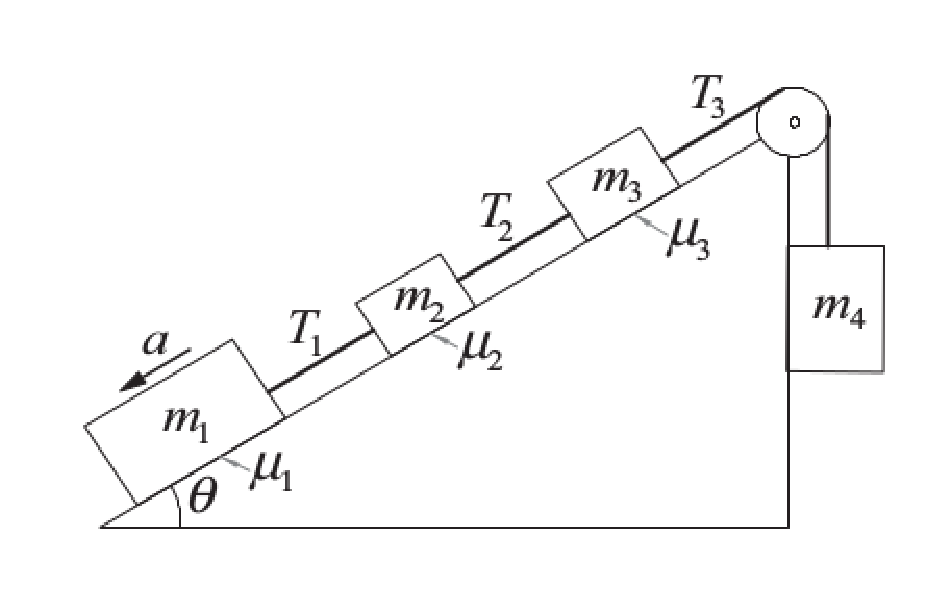
\includegraphics[scale=0.75]{Imagenes/EjercicioMasas.eps}
\end{figure}
Las ecuaciones de movimiento de los bloques son las siguientes:
\begin{align*}
T_{1} + m_{1} \: a &= m_{1} \: g \: (\sin \theta - \mu_{1} \: \cos \theta) \\
-T_{1} + T_{2} + m_{2} \: a &= m_{2} \: g \: (\sin \theta - \mu_{2} \: \cos \theta) \\
-T_{2} + T_{3} + m_{3} \: a &= m_{3} \: g \: (\sin \theta - \mu_{3} \: \cos \theta) \\
-T_{3} + m_{4} \: a &= m_{4} \: g
\end{align*}
donde las $T_{i}$ representan las fuerzas de tensión en las cuerdas y $a$ es la aceleración del sistema.
\par
Calcula $a$ y $T_{i}$ si $\theta=\SI{45}{\degree}$, $g=\SI{9.82}{\meter\per\square\second}$
\item Resolver las siguientes ecuaciones simétricas tridiagonales
\[ \begin{split}
4 x_{1} - x_{2} =& \: 9 \\
-x_{i-1} + 4x_{i} - x_{i+1} =& \: 5, \hspace{1cm} i = 2, \ldots, n-1 \\
-x_{n-1} + 4 x_{n} =& \: 5
\end{split} \]
con $n=10$.
% \item El sistema mostrado en la figura consiste en $n$ resortes lineales que soportan $n$ masas. La constante de los resortes se indican por $k_{i}$, mientras que el peso de las masas, es $W_{i}$ y $x_{i}$ son los desplazamientos de las masas (medidos de la posición donde el resorte no está deformado). La llamada \emph{formulación de desplazamiento} se obtiene escribiendo la ecuación de equilibrio para cada masa y sustituyendo $F_{i} = k_{i}(x_{i+1}-x_{i})$ para la fuerza en los resortes. El resultado es un conjunto de ecuaciones simétricas y tridiagonal:
% \par
% \begin{minipage}{0.5\textwidth}
% \[ \begin{split}
% (k_{1} + k_{2})x_{1} - k_{2}x_{2} =& W_{1} \\
% -k_{i} x_{i-1} + (k_{i} + k_{i+1}) x_{i} - k_{i+1} x_{i+1} =& W_{i}, \hspace{1cm} i=2,3,\ldots,n-1 \\
% -k_{n} x_{n-1} + k_{n} x_{n} =& W_{n}
% \end{split} \]
% \end{minipage}
% \begin{minipage}{0.5\textwidth}
% \begin{figure}[H]
% \centering
% \begin{tikzpicture}
% \tikzstyle{spring}=[thick,decorate,decoration={zigzag,pre length=0.1cm,post
%   length=0.1cm,segment length=6}]
% 	\draw (0,0) [pattern=north west lines] rectangle(1,0.25);
% 	\draw [spring](0.5,0) -- (0.5,-1) node [midway, right=0.4cm] {$k_{1}$}; 
% 	\draw (0,-1) rectangle node {$W_{1}$} (1,-2);
% 	\draw (1,-1) -- (1.5,-1);
% 	\draw [->]  (1.3,-1) -- node [near end, right=0.2]{$x_{1}$}(1.3,-1.7); 
% 	\draw [spring](0.5,-2) -- (0.5,-3) node [midway, right=0.4cm] {$k_{2}$};
% 	\draw (0,-3) rectangle node {$W_{2}$} (1,-4);
% 	\draw (1,-3) -- (1.5,-3);
% 	\draw [->]  (1.3,-3) -- node [near end, right=0.2]{$x_{2}$}(1.3,-3.7); 
% 	\draw [spring](0.5,-4) -- (0.5,-5) node [midway, right=0.4cm] {$k_{3}$};
% 	\draw (0.5,-5.1) node {$\vdots$};
% 	\draw [spring](0.5,-5.5) -- (0.5,-6.5) node [midway, right=0.4cm] {$k_{n}$};
% 	\draw (0,-6.5) rectangle node {$W_{n}$} (1,-7.5);
% 	\draw (1,-6.5) -- (1.5,-6.5);
% 	\draw [->]  (1.3,-6.5) -- node [near end, right=0.2]{$x_{n}$}(1.3,-7.2); 
% \end{tikzpicture}
% \end{figure}
% \end{minipage}
% Escribe un programa que resuelva este conjunto de ecuaciones para los valores dados de $n$, $k$ y $W$. Considera $n=5$ y 
% \[ \begin{split} 
% k_{1} = k_{2} = k_{3} = 10 \mbox{ N/mm} \hspace{2cm} k_{4} = k_{5} = 5 \mbox{ N/mm} \\
% W_{1} = W_{3} = W_{5} = 100 \mbox{ N} \hspace{2cm} W_{2} = W_{4} = 50 \mbox{ N}
% \end{split} \]

\end{enumerate}	
\end{document}